\acrfull{HTB}\cite{htb} (figura \ref{fig:htb-logo}) es una plataforma online gratuita que une a cientos de miles de hackers. En el núcleo de \acrshort{HTB} hay una red de máquinas vulnerables listas para ser atacadas y para que se practiquen las habilidades de ciberseguridad, de forma totalmente legal. El objetivo es realizar un \acrshort{CTF}, es decir, conseguir ser root para demostrar que has conseguido el control total sobre la máquina.\\

\begin{figure}[h]
    \centering
    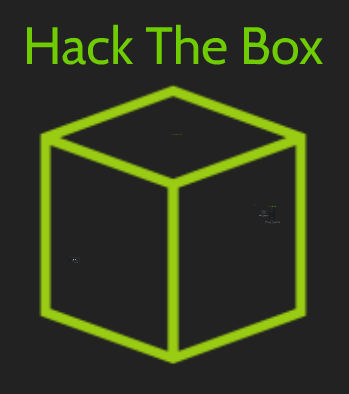
\includegraphics[width=0.20\textwidth]{images/sections/stateOfTheArt/htb-logo.png}
    \caption{Logo de \textit{\acrshort{HTB}}}
    \label{fig:htb-logo}
\end{figure}

En \acrshort{HTB} hay distintos desafíos, como \textit{machines}, \textit{challenges}, \textit{tracks} y más, cada uno con distintos niveles de dificultad (``\textit{easy}``, ``\textit{medium}``, ``\textit{hard}`` e ``\textit{insane}``), además de un \textit{Starting Point} para personas que se enfrenten por primera vez a este tipo de desafíos. Cada desafío proporciona una serie de puntos que sirven para escalar en el \textit{ranking} global.

\acrshort{HTB} tiene una subscripción de pago que te permite acceder a las máquinas retiradas, además de proporcionarte más características, como laboratorios VIP o acceso a \textit{write-ups} oficiales.\\

A continuación se mencionan los principales laboratorios en \acrshort{HTB}.

\subsubsection{Challenges}
Los desafíos (\textit{challenges}) están categorizados por su temática, como se muestra en la figura \ref{fig:htb-challenges}. Cada desafío tiene una dificultad, y se centra en resolver el desafío para encontrar el flag pertinente.

\begin{figure}[h]
    \centering
    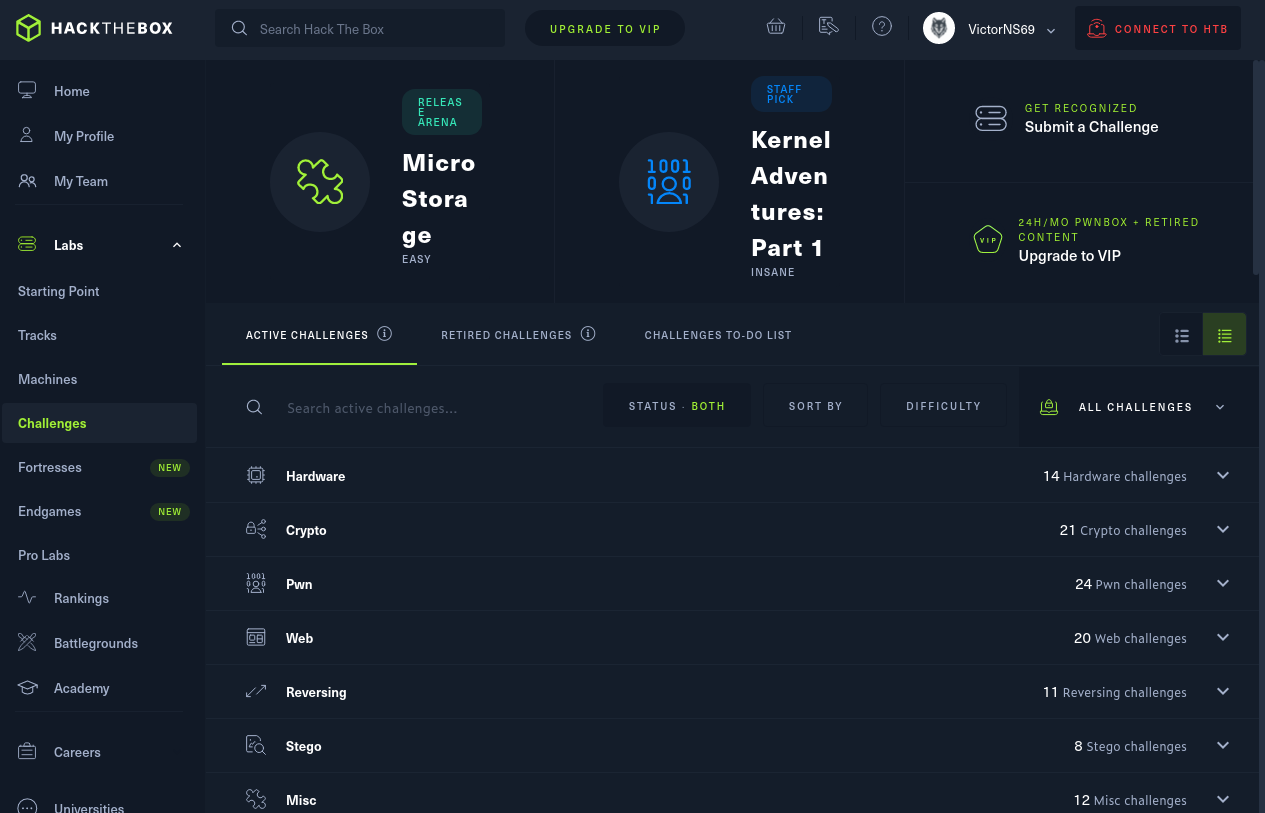
\includegraphics[width=0.7\textwidth]{images/sections/stateOfTheArt/htb-challenges.png}
    \caption{Tipos de \textit{challenges} en \textit{\acrshort{HTB}}}
    \label{fig:htb-challenges}
\end{figure}

\subsubsection{Machines}
Las máquinas (\textit{machines}) intentan simular en mayor o menor medida a un servidor real, con páginas web, servicios de administración como \acrshort{ssh} o \textit{telnet}, descarga y subida de ficheros a través de \acrshort{ftp}, servidores de dominio Window, etc. Para poder conseguir ser root se tendrán que usar técnicas de escalada de privilegios, esteganografía, fuerza bruta, exploits, análisis de código y cualquier conocimiento del mundo de la ciberseguridad. En la figura \ref{fig:htb-machines} se pueden ver las máquinas disponibles a fecha de la realización de este trabajo. Las máquinas van desapareciendo y van naciendo máquinas nuevas con el paso del tiempo.\\

\begin{figure}[h]
    \centering
    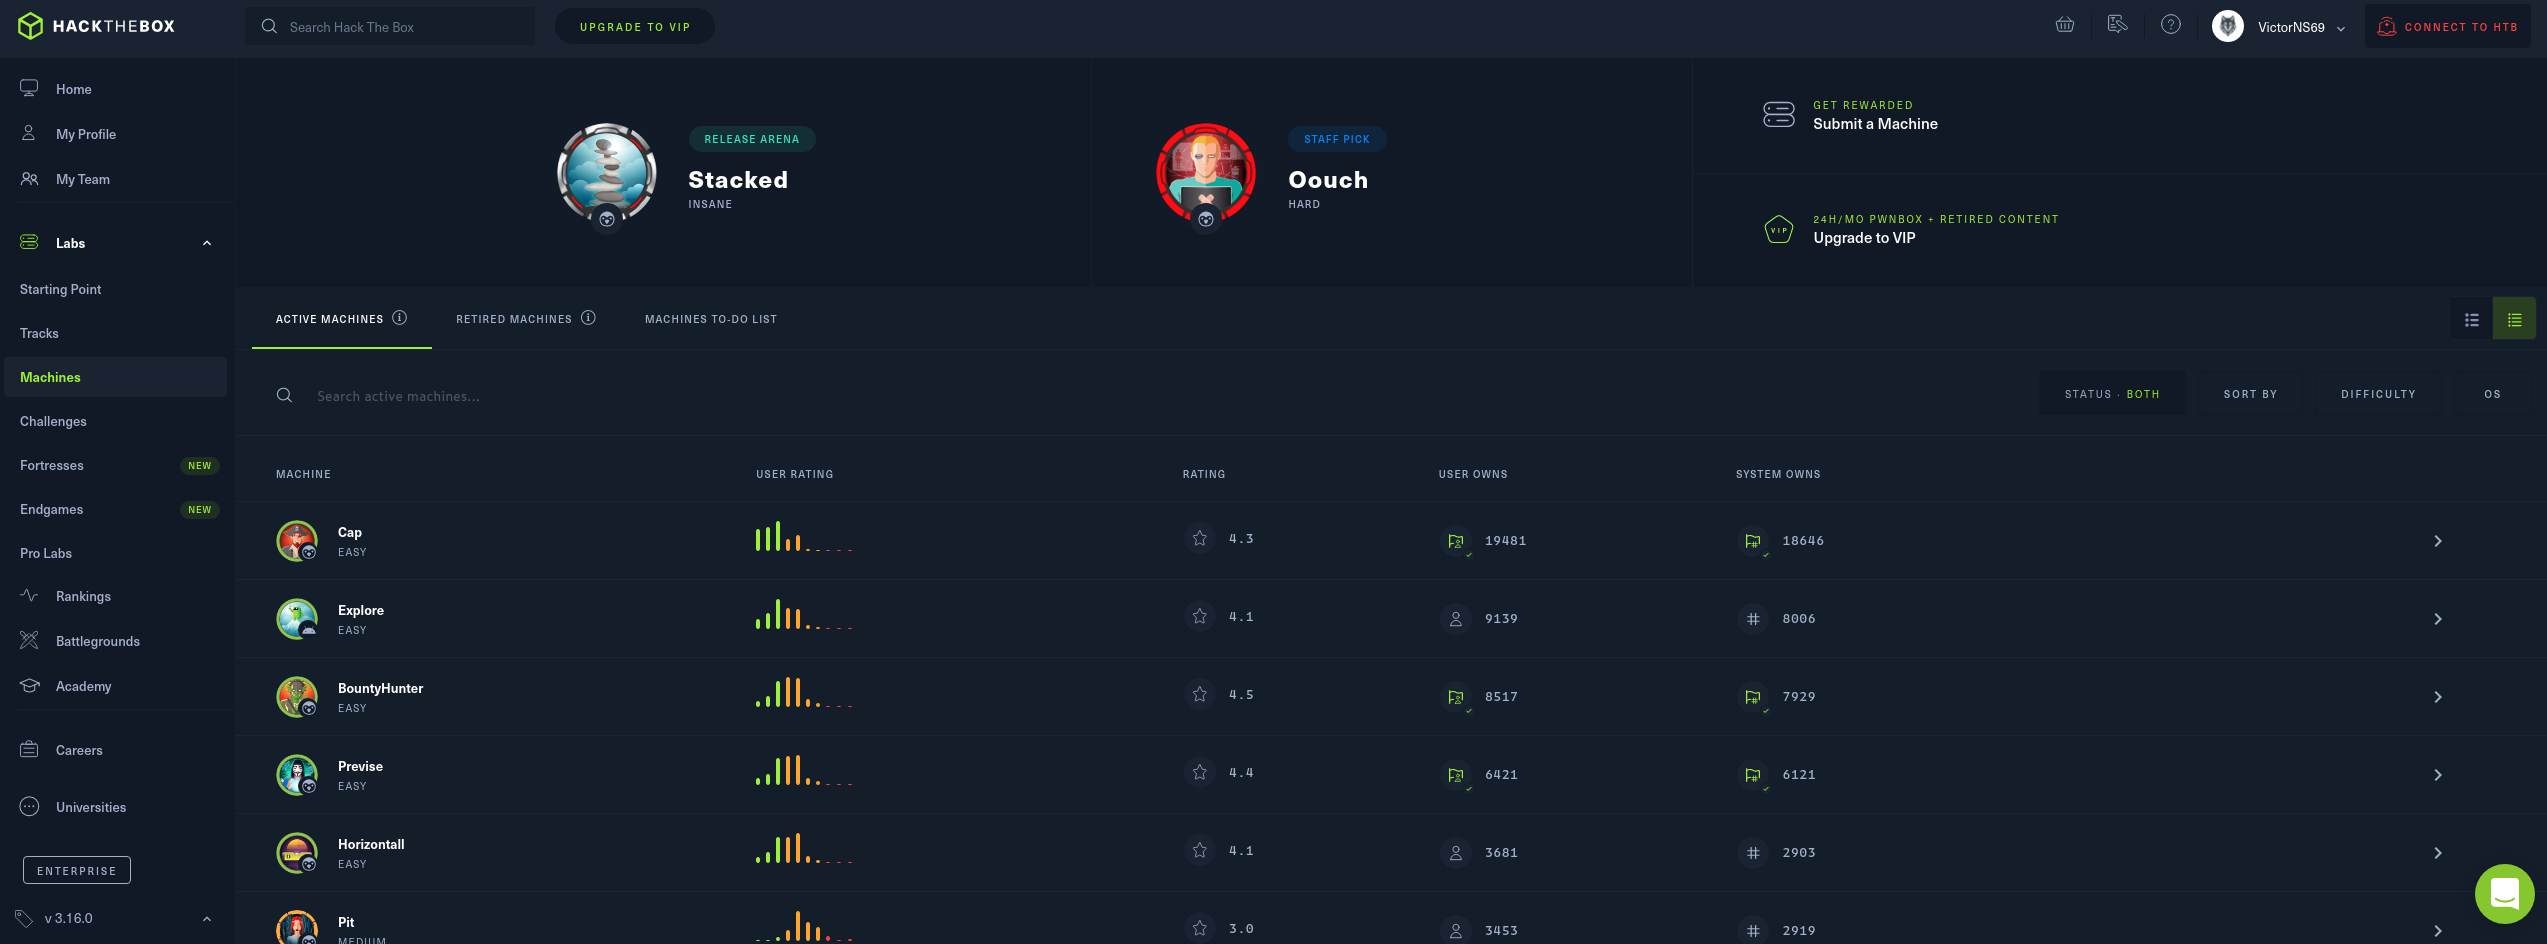
\includegraphics[width=1.0\textwidth]{images/sections/stateOfTheArt/htb-machines.png}
    \caption{\textit{Machines} en \textit{\acrshort{HTB}}}
    \label{fig:htb-machines}
\end{figure}

\subsubsection{Tracks}
Un \textit{Track} es un conjunto de máquinas y desafíos enlazados entre sí, centradas en un objetivo o tecnología concreta, que permite al usuario profundizar sobre ese tema en concreto. En la siguiente figura (figura \ref{fig:htb-tracks}) se puede ver el primer \textit{track} disponible.
\begin{figure}[h]
    \centering
    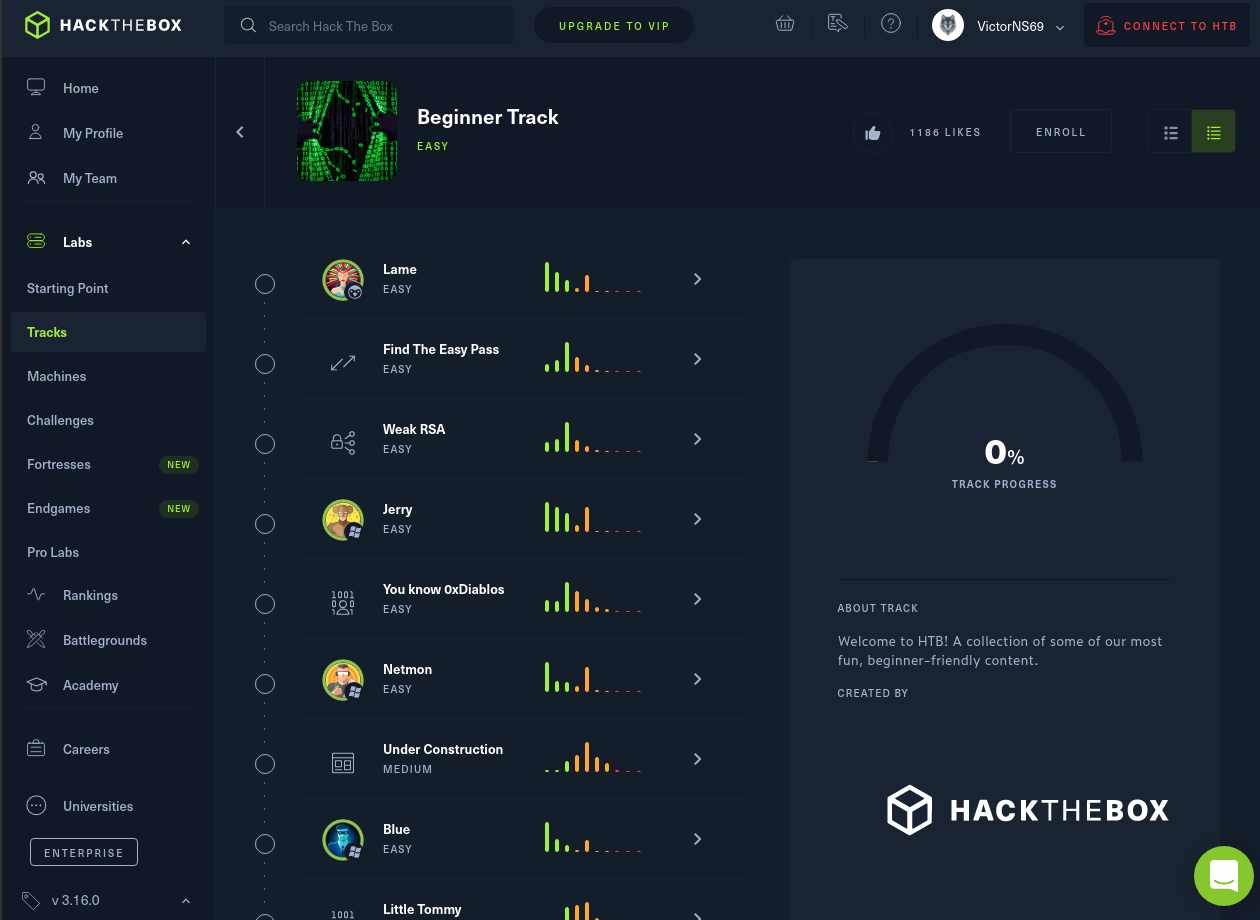
\includegraphics[width=0.6\textwidth]{images/sections/stateOfTheArt/htb-tracks.png}
    \caption{\textit{Beginner Track} en \textit{\acrshort{HTB}}}
    \label{fig:htb-tracks}
\end{figure}

\subsubsection{Endgames}
La sección \textit{endgames} de \acrshort{HTB} son una serie de laboratorios avanzados simulando escenarios e infraestructuras del mundo real. El objetivo, al igual que con las \textit{machines} es obtener el flag de \textit{root}, pero en estos laboratorios hay más máquinas, redes más complejas y un desafío mucho mayor.\\

Para desbloquear el \textit{endgame}, se tiene que haber alcanzado un rango mínimo en \acrshort{HTB} de ``\textit{Guru}``. El rango se consigue realizando máquinas, desafíos y demás.
